\documentclass[border=5pt]{standalone}
\usepackage{tikz}
\usetikzlibrary{positioning, arrows.meta, shapes.geometric, calc, fit, backgrounds}
\usepackage{amsmath,amssymb}

\begin{document}
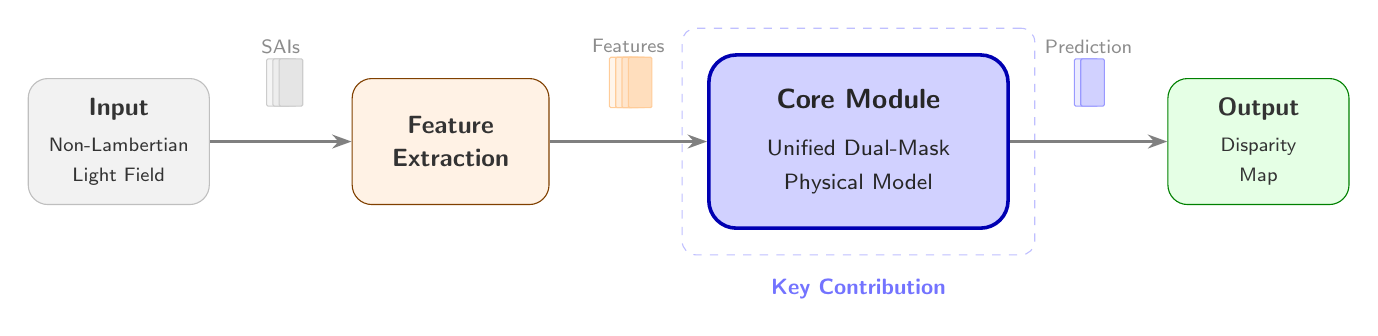
\begin{tikzpicture}[
  inp/.style={
    draw=gray!50, fill=gray!10, rounded corners=2.5mm,
    minimum width=2.3cm, minimum height=1.6cm,
    align=center, font=\sffamily\small, text=black!80
  },
  proc/.style={
    draw=orange!50!black, fill=orange!10, rounded corners=2.5mm,
    minimum width=2.5cm, minimum height=1.6cm,
    align=center, font=\sffamily\small, text=black!80
  },
  innov/.style={
    draw=blue!70!black, fill=blue!18, rounded corners=3.5mm,
    minimum width=3.8cm, minimum height=2.2cm,
    line width=1.3pt,
    align=center, font=\sffamily, text=black!85
  },
  outp/.style={
    draw=green!50!black, fill=green!10, rounded corners=2.5mm,
    minimum width=2.3cm, minimum height=1.6cm,
    align=center, font=\sffamily\small, text=black!80
  },
  arr/.style={-{Stealth[length=7pt, width=5pt]}, line width=1.1pt, color=black!50},
  lbl/.style={font=\sffamily\scriptsize, text=black!45},
]

% ===== Main Pipeline =====
\node[inp] (m1) {\textbf{Input}\\[2pt]{\scriptsize Non-Lambertian}\\{\scriptsize Light Field}};

\node[proc, right=1.8cm of m1] (m2) {\textbf{Feature}\\[1pt]\textbf{Extraction}};

\node[innov, right=2.0cm of m2] (m3)
  {{\normalsize\bfseries Core Module}\\[5pt]{\footnotesize\mdseries Unified Dual-Mask}\\{\footnotesize\mdseries Physical Model}};

\node[outp, right=2.0cm of m3] (m4) {\textbf{Output}\\[2pt]{\scriptsize Disparity}\\{\scriptsize Map}};

% ===== Feature map mini-icons above arrows =====
% Between m1 and m2
\begin{scope}[shift={($(m1.east)!0.5!(m2.west)+(0,0.75)$)}]
  \draw[draw=gray!40, fill=gray!8, rounded corners=0.5pt] (-0.18,-0.3) rectangle (0.12,0.3);
  \draw[draw=gray!40, fill=gray!14, rounded corners=0.5pt] (-0.10,-0.3) rectangle (0.20,0.3);
  \draw[draw=gray!40, fill=gray!20, rounded corners=0.5pt] (-0.02,-0.3) rectangle (0.28,0.3);
\end{scope}
\node[lbl] at ($(m1.east)!0.5!(m2.west)+(0,1.2)$) {SAIs};

% Between m2 and m3
\begin{scope}[shift={($(m2.east)!0.5!(m3.west)+(0,0.75)$)}]
  \draw[draw=orange!40, fill=orange!8, rounded corners=0.5pt] (-0.24,-0.32) rectangle (0.06,0.32);
  \draw[draw=orange!40, fill=orange!14, rounded corners=0.5pt] (-0.16,-0.32) rectangle (0.14,0.32);
  \draw[draw=orange!40, fill=orange!20, rounded corners=0.5pt] (-0.08,-0.32) rectangle (0.22,0.32);
  \draw[draw=orange!40, fill=orange!26, rounded corners=0.5pt] (0.0,-0.32) rectangle (0.30,0.32);
\end{scope}
\node[lbl] at ($(m2.east)!0.5!(m3.west)+(0,1.22)$) {Features};

% Between m3 and m4
\begin{scope}[shift={($(m3.east)!0.5!(m4.west)+(0,0.75)$)}]
  \draw[draw=blue!40, fill=blue!8, rounded corners=0.5pt] (-0.18,-0.3) rectangle (0.12,0.3);
  \draw[draw=blue!40, fill=blue!18, rounded corners=0.5pt] (-0.10,-0.3) rectangle (0.20,0.3);
\end{scope}
\node[lbl] at ($(m3.east)!0.5!(m4.west)+(0,1.2)$) {Prediction};

% ===== Arrows =====
\draw[arr] (m1) -- (m2);
\draw[arr] (m2) -- (m3);
\draw[arr] (m3) -- (m4);

% ===== Highlight on core module =====
\begin{scope}[on background layer]
  \node[draw=blue!25, dashed, rounded corners=5pt, inner sep=9pt,
        fit=(m3)] (hl) {};
\end{scope}
\node[font=\sffamily\footnotesize\bfseries, text=blue!55]
  at (hl.south) [below=5pt, anchor=north] {Key Contribution};

\end{tikzpicture}
\end{document}